\begin{example}~
\label{ex:multiple_noisy}
	Consider the communication of \AgentOne and \AgentTwo via covert channels. Let the confidential information be represented by $P = \set{(1,3),(2,1),(3,4),\\(4,1),(5,5),(6,9)}$. Suppose the \AgentOne and \AgentTwo devise a scheme for transmitted the confidential information involving multiple channels and the addition of noise to the channels. The two agents decide that they are going to split the confidential over two covert channels where on the first channel they will send the information corresponding to the odd times as $Q_1 = \set{(1,12),(3,16),(5,17)}$ and on the second channel they will send the information corresponding to the even times as  $Q_2 = \set{(2,1),(4,1),(6,18)}$. For each channel, \AgentOne adds noise to the communication channel by some noise relations represented by $S_1$ and $S_2$. \newline 

	We define the relations $P$, $Q_1$ and $Q_2$ in \relview\ as follows: \newpage

	\begin{figure}[ht]
		\centering
		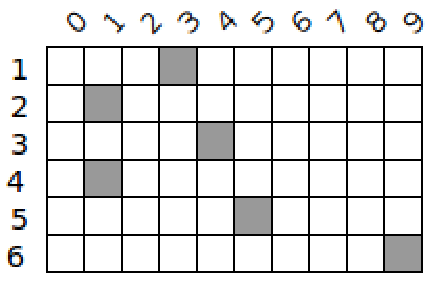
\includegraphics[scale=0.65]{Figures/PDF/Relview/P.pdf}
		\caption{Relation $P$ for Example~\ref{ex:multiple_noisy}.}
		\label{fig:multiple_noisy_p}
	\end{figure}
	
	\begin{figure}[ht]
		\centering
		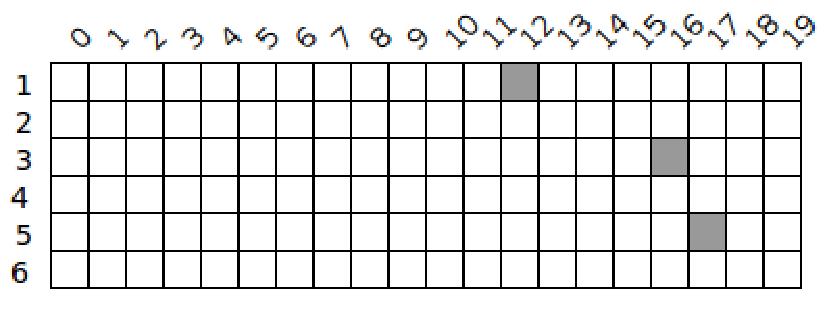
\includegraphics[scale=0.65]{Figures/PDF/Relview/Q1.pdf}
		\caption{Relation $Q_1$ for Example~\ref{ex:multiple_noisy}.}
		\label{fig:multiple_noisy_q1}
	\end{figure}

	\begin{figure}[ht]
		\centering
		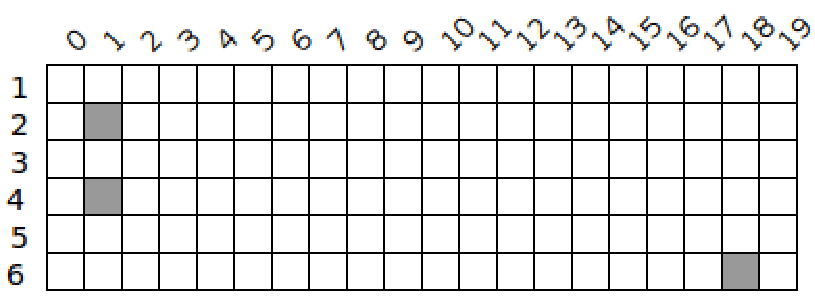
\includegraphics[scale=0.65]{Figures/PDF/Relview/Q2.pdf}
		\caption{Relation $Q_2$ for Example~\ref{ex:multiple_noisy}.}
		\label{fig:multiple_noisy_q2}
	\end{figure}

	Let the noise relations represented by $S_1$ and $S_2$ be defined as follows: \newpage

	\begin{figure}[ht]
		\centering
		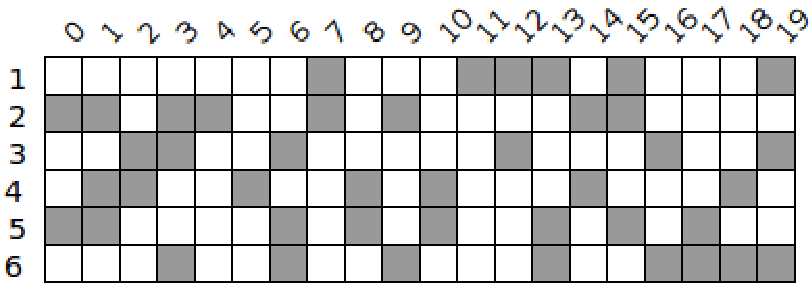
\includegraphics[scale=0.65]{Figures/PDF/Relview/NoiseQ1.pdf}
		\caption{Noise relation $S_1$ for Example~\ref{ex:multiple_noisy}.}
		\label{fig:multiple_noisy_s1}
	\end{figure}
	
	\begin{figure}[ht]
		\centering
		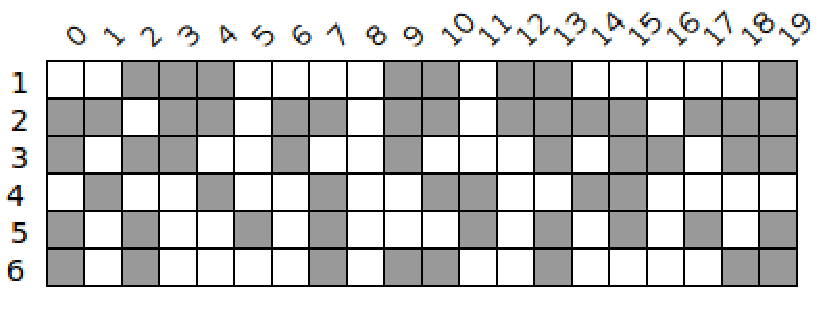
\includegraphics[scale=0.65]{Figures/PDF/Relview/NoiseQ2.pdf}
		\caption{Noise relation $S_2$ for Example~\ref{ex:multiple_noisy}.}
		\label{fig:multiple_noisy_s2}
	\end{figure}
	
	We assume that the noise is added to the communication channel by the union operation ( $\!\!\!\STjoin\!\!\!$ ) and that the channels are combined using the intersection operation ( $\!\!\!\STmeet\!\!\!$ ). The relation representing the combination of the noisy channels is then as follows: \newline

	\begin{figure}[ht]
		\centering
		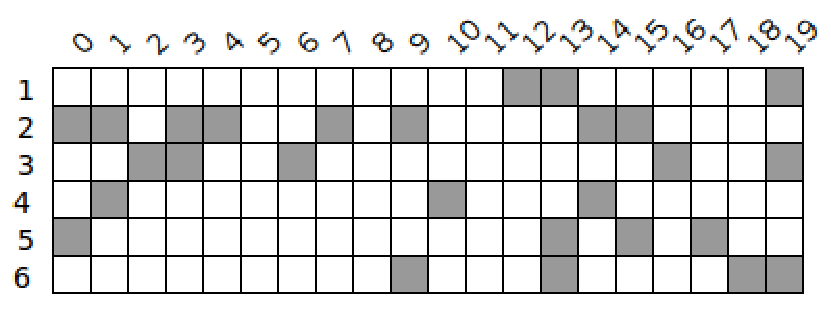
\includegraphics[scale=0.65]{Figures/PDF/Relview/NoiseCombine.pdf}
		\caption{Relation $(Q_1 \STjoin S_1) \STmeet (Q_2 \STjoin S_2)$ for Example~\ref{ex:multiple_noisy}.}
		\label{fig:multiple_noisy_combine}
	\end{figure}	

	We verify the existence of an abstraction relation by executing Program~\ref{prog:test} ($Result = Test(P, (Q_1 \STjoin S_1) \STmeet (Q_2 \STjoin S_2))$). \newline

	\begin{figure}[ht]
		\centering
		
\includegraphics[scale=0.65]{Figures/PDF/Relview/True.pdf}
		\caption{Relation $Result$ for Example~\ref{ex:multiple_noisy}.}
		\label{fig:multiple_noisy_result}
	\end{figure}

	Therefore, the test has passed so we can compute the abstraction relation by executing Program~\ref{prog:compute} ($X = Compute(P,(Q_1 \STjoin S_1) \STmeet (Q_2 \STjoin S_2),R)$) where $R$ is the filtering relation. \newline

	\begin{figure}[ht]
		\centering
		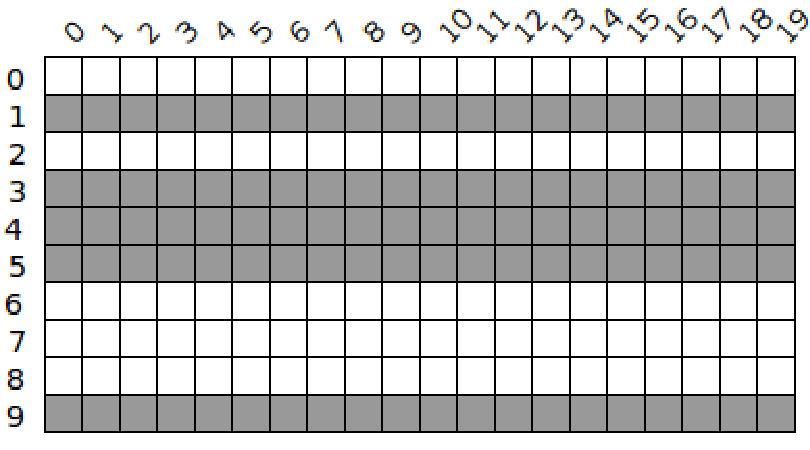
\includegraphics[scale=0.65]{Figures/PDF/Relview/R.pdf}
		\caption{Filtering relation $R$ for Example~\ref{ex:multiple_noisy}.}
		\label{fig:multiple_noisy_r}
	\end{figure}

	\begin{figure}[ht]
		\centering
		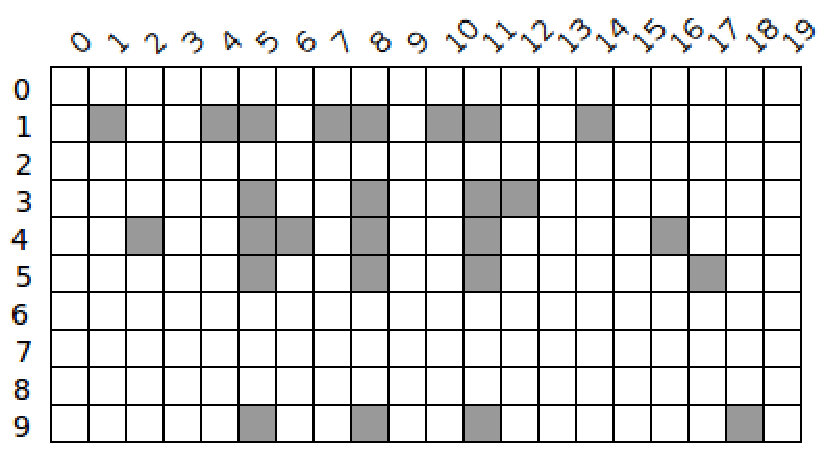
\includegraphics[scale=0.65]{Figures/PDF/Relview/XX.pdf}
		\caption{Abstraction $X$ for Example~\ref{ex:multiple_noisy}.}
		\label{fig:multiple_noisy_x}
	\end{figure}
	
\end{example}